\documentclass{beamer}

\usepackage{graphicx}
\usetheme{CambridgeUS}


\definecolor{myyellow}{RGB}{255, 255, 0}  % Define yellow color
\definecolor{mygreen}{RGB}{0, 255, 150}    % Define green color

\title{Environmental Pollution}
\subtitle{Causes, Effects, and Solutions}
\author{Masud Rana}
\date{\today}

\begin{document}

{
\setbeamercolor{background canvas}{bg=mygreen}
\begin{frame}
  \titlepage
\end{frame}
}


\begin{frame}{Table of Contents}
  \tableofcontents
\end{frame}

\section{Introduction}
\begin{frame}{What is Environmental Pollution?}
  \begin{itemize}
    \item \textcolor{myyellow}{Introduction to Pollution The presence of harmful substances in the environment.}
    \item \textcolor{mygreen}{Types of pollution: air, water, soil, noise, etc.}
  \end{itemize}
\end{frame}

\section{Causes of Pollution}
\begin{frame}{Major Causes of Pollution}
  \begin{itemize}
    \item Industrial emissions
    \item Vehicle exhaust
    \item Deforestation
    \item Plastic waste
    \item Overpopulation
  \end{itemize}
\end{frame}

\section{Effects of Pollution}
\begin{frame}{Impact on the Environment and Health}
  \begin{columns}
    \column{0.5\textwidth}
    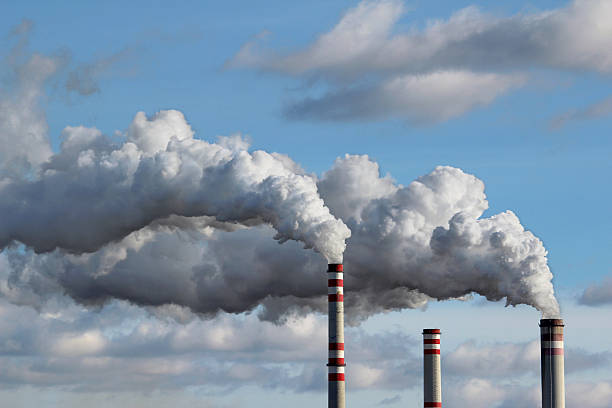
\includegraphics[width=\textwidth]{images/air-pollution.png}
    \column{0.5\textwidth}
    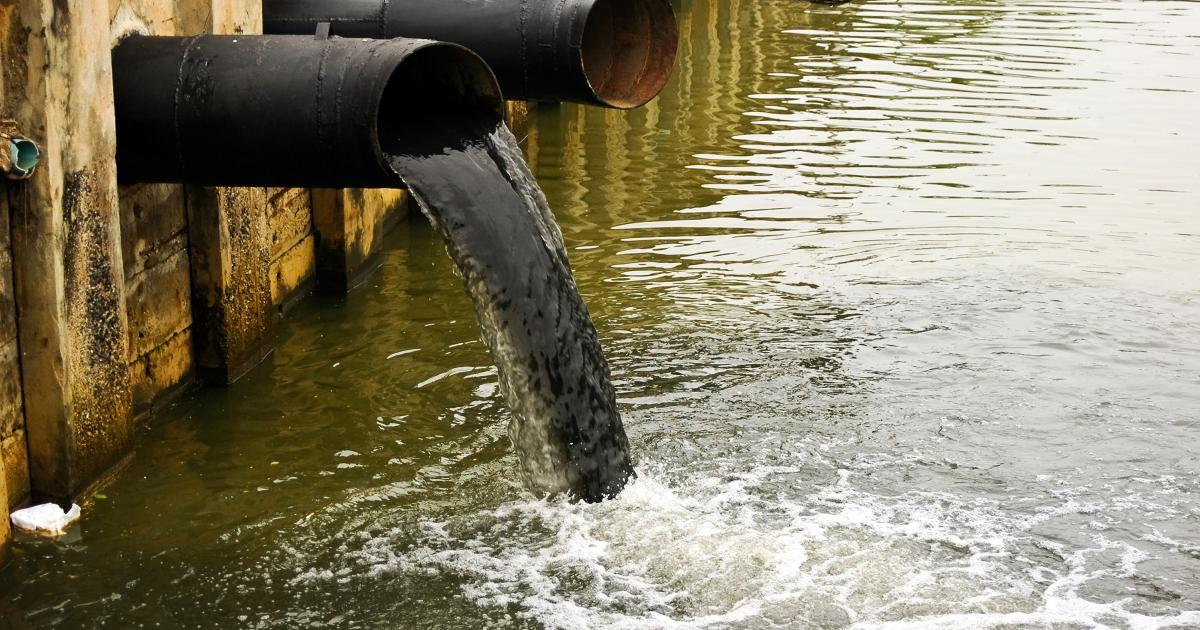
\includegraphics[width=\textwidth]{images/water-pollution.png}
  \end{columns}

  \begin{columns}
    \column{0.5\textwidth}
    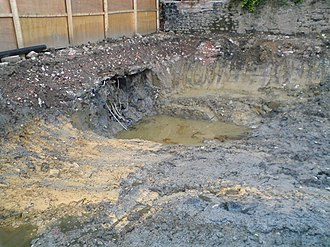
\includegraphics[width=\textwidth]{images/soil-pollution.png}
    \column{0.5\textwidth}
    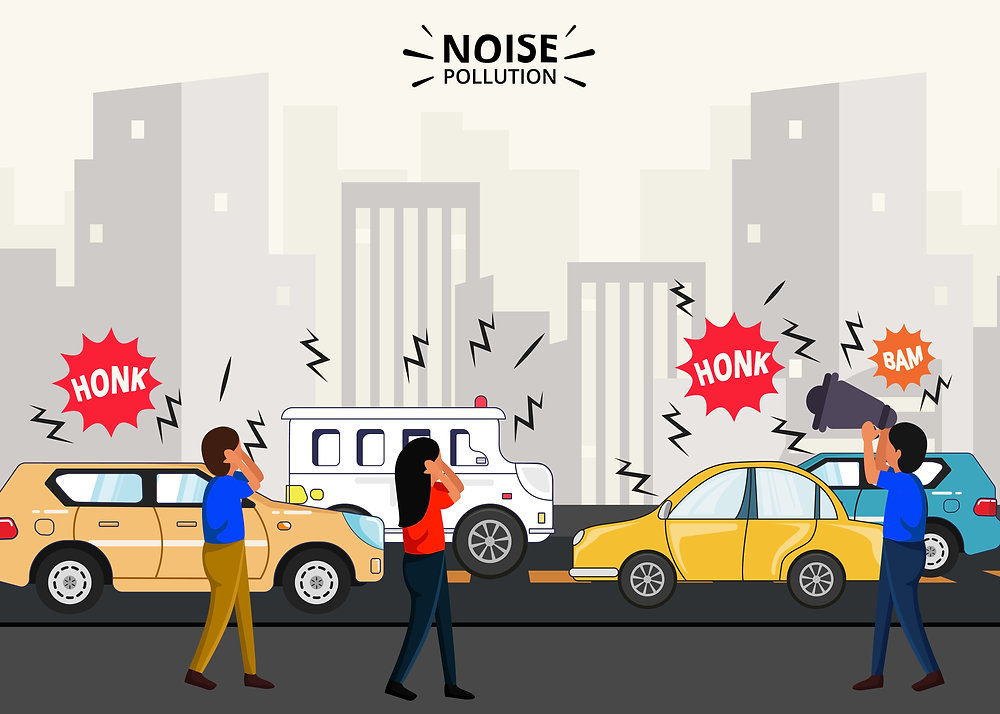
\includegraphics[width=\textwidth]{images/noise-pollution.png}0
  \end{columns}
\end{frame}

\begin{frame}{Insight into Global Pollution}
  \begin{table}[]
    \centering
    \setlength{\tabcolsep}{5pt} 
    \begin{tabular}{|p{0.25\textwidth}|p{0.35\textwidth}|p{0.25\textwidth}|}
      \hline
      \textbf{Type of Pollution} & \textbf{Global Impact} & \textbf{Major Contributors} \\
      \hline
      Air Pollution & Climate change, health issues & Industries, vehicles \\
      \hline
      Water Pollution & Contaminated drinking water & Factories, agriculture \\
      \hline
      Soil Pollution & Loss of fertility, toxic crops & Pesticides, landfills \\
      \hline
      Noise Pollution & Hearing loss, stress & Urban areas, traffic \\
      \hline
    \end{tabular}
    \caption{Global Insights into Different Types of Pollution}
  \end{table}
\end{frame}


\section{Solutions to Pollution}
\begin{frame}{How Can We Reduce Pollution?}
  \begin{enumerate}
    \item Adopting renewable energy sources.
    \item Recycling and waste management.
    \item Reducing deforestation and planting trees.
    \item Implementing stricter environmental laws.
    \item Raising awareness and education.
  \end{enumerate}
\end{frame}


\section{Conclusion}
\begin{frame}{Final Thoughts}
  \begin{itemize}
    \item Environmental pollution is a critical issue.
    \item Collective efforts are essential to mitigate its effects.
    \item Sustainable practices and innovation are key.
  \end{itemize}
\end{frame}

\begin{frame}
  \centering
  \LARGE{Thank You!} \vspace{1cm} \\
  \normalsize{Questions?}
  \footnote{Source: Blog,\url{https://example.com/blog/first/211}}.
\end{frame}

\end{document}
